\documentclass{jsarticle}
\usepackage[dvipdfmx]{graphicx}
\usepackage{listings}
\usepackage{afterpage}
\begin{document}
\title{課題9 ノイズ除去}
\author{13EC060 武澤 裕介}
\maketitle
\begin{abstract}
matlabを用いてフィルタによるノイズ除去を行い考察する。
\end{abstract}
\section{ノイズ除去}
まず、今回使用する原画像を図1に示す。


\begin{figure}[htbp]
 \begin{center}
  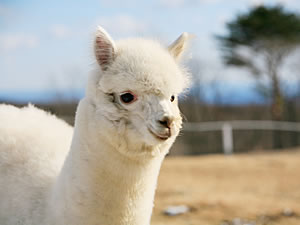
\includegraphics[width=5cm,height=5cm]{a.jpg}
 \end{center}
 \caption{原画像}
\end{figure}

\begin{lstlisting}[basicstyle=\ttfamily\footnotesize, frame=single]
filename = uigetfile('*');
ORG=imread(filename); % 原画像の入力
ORG = rgb2gray(ORG); colormap(gray); colorbar;
imagesc(ORG); axis image; % 画像の表示
pause; % 一時停止
 \end{lstlisting}
を用いてまず入力画像のグレースケール画像を表示させる。

\newpage
\begin{figure}[htbp]
 \begin{center}
  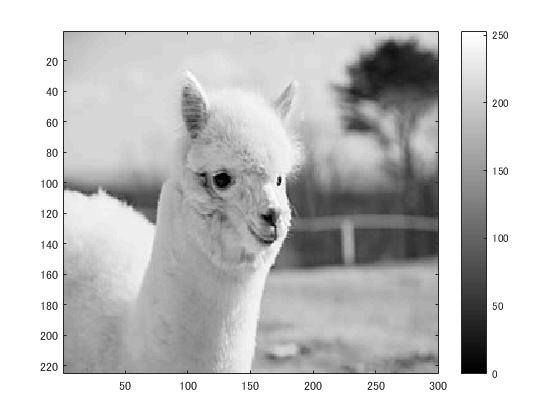
\includegraphics[width=10cm]{8-0.jpg}
 \end{center}
 \caption{グレースケール画像}
\end{figure}

次に
\begin{lstlisting}[basicstyle=\ttfamily\footnotesize, frame=single]
ORG = imnoise(ORG,'salt & pepper',0.02); % ノイズ添付
imagesc(ORG); colormap(gray); colorbar; % 画像の表示
pause;
 \end{lstlisting}
を用いて画像にノイズを添付する。

\newpage
\begin{figure}[htbp]
 \begin{center}
  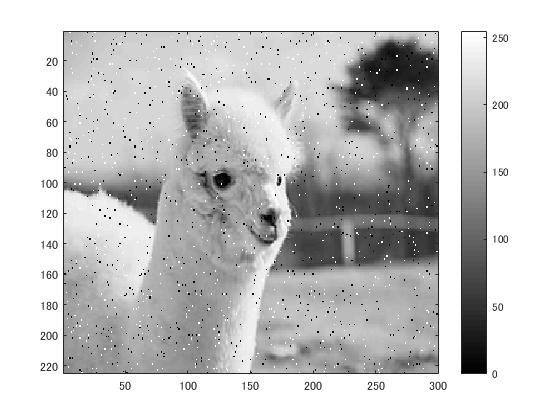
\includegraphics[width=10cm]{8-1.jpg}
 \end{center}
 \caption{ノイズ添付画像}
\end{figure}

最後に
\begin{lstlisting}[basicstyle=\ttfamily\footnotesize, frame=single]
IMG = filter2(fspecial('average',3),ORG); % 平滑化フィルタで雑音除去
imagesc(IMG); colormap(gray); colorbar; % 画像の表示
pause;
IMG = medfilt2(ORG,[3 3]); % メディアンフィルタで雑音除去
imagesc(IMG); colormap(gray); colorbar; % 画像の表示
pause;
f=[0,-1,0;-1,5,-1;0,-1,0]; % フィルタの設計
IMG = filter2(f,IMG,'same'); % フィルタの適用
imagesc(IMG); colormap(gray); colorbar; % 画像の表示
pause;
 \end{lstlisting}
を用いてそれぞれのフィルタを適応した画像を表示する。

\newpage
\begin{figure}[htbp]
 \begin{center}
  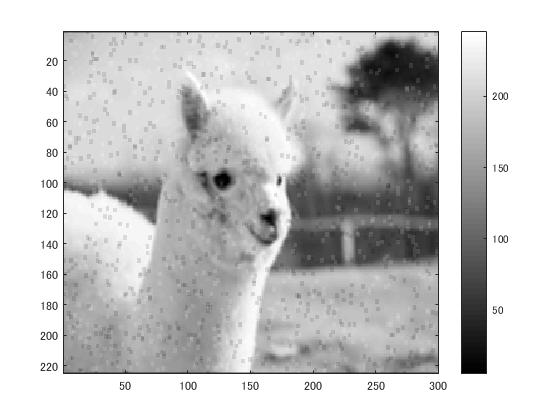
\includegraphics[width=10cm]{8-2.jpg}
 \end{center}
 \caption{平滑化フィルタ}
\end{figure}

\newpage
\begin{figure}[htbp]
 \begin{center}
  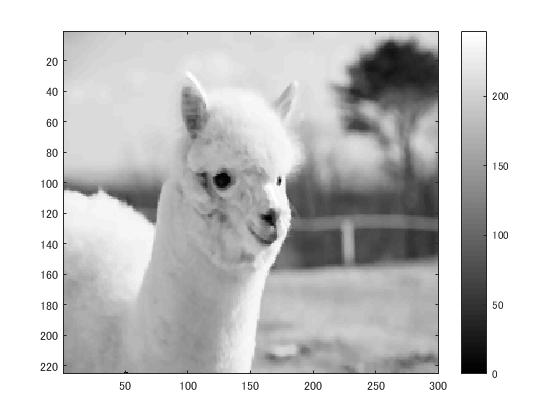
\includegraphics[width=10cm]{8-3.jpg}
 \end{center}
 \caption{メディアンフィルタ}
\end{figure}

\newpage
\begin{figure}[htbp]
 \begin{center}
  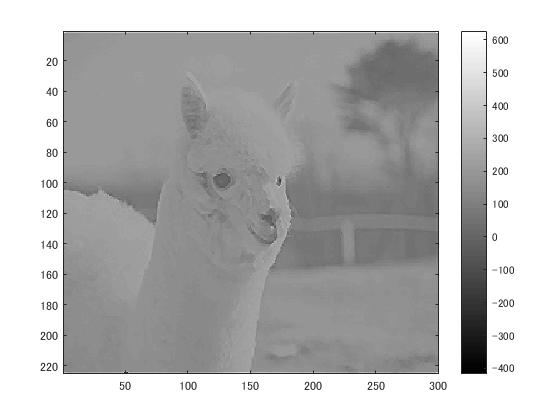
\includegraphics[width=10cm]{8-4.jpg}
 \end{center}
 \caption{設計したフィルタ}
\end{figure}

\section{考察}
画像にノイズを添付して、フィルタを通してノイズを除去した、移動平均フィルタではノイズは除去しきれなかったが、他の2つのフィルタではノイズを除去できた。

\end{document}